\documentclass[hyperref={urlcolor=black, citecolor=black, pdfpagemode=UseNone, pdfpagelayout=SinglePage, pdfstartview=}]{beamer}
%\usepackage[EU1]{fontenc}
\usepackage{ru}
\usepackage{lmodern}
\usepackage{url}
\usepackage[british]{babel}
\usepackage{tikz}
\usepackage{fontspec}
%\usepackage{graphicx}
%\usepackage{amsfonts}
%\usepackage{wrapfig}
%\usepackage{booktabs}
\usepackage{expdlist}

\mode<presentation>
\usetheme{Darmstadt}
\usefonttheme[onlysmall]{structurebold}

\newfontfamily\RUfontbold[]{ITCMendozaRoman LT Medium}
\newfontfamily\RUfont[]{ITCMendozaRoman LT Book}


\title[IRMA Verified Assurer]{IRMA Verified Assurer}
\subtitle{Securely storing identity document chip data onto IRMA cards}
\author[Geert Smelt]{Geert Smelt}
\institute[Radboud University Nijmegen]{{\RUfontbold Radboud University Nijmegen}\\Kerckhoff's Institute}
\date[2015/11/06]{November 6$^{\textnormal{th}}$, 2015}


\begin{document}

\begin{frame}
  \titlepage
\end{frame}

\begin{frame}
  \frametitle{Outline}
  \tableofcontents%[pausesections]
\end{frame}

\section{Introduction}
\begin{frame}
  \frametitle{Authentication}
  \begin{columns}
    \column{0.55\textwidth}    
    \begin{itemize}
      \item<1-> Gain access to a restricted product or service
      \begin{itemize}
        \item<1-> {\scriptsize No selling of alcohol or cigarettes to minors}
        \item<1-> {\scriptsize Verification required}
      \end{itemize}
      \item<2-> Passport
      \begin{itemize}
        \item<2-> {\scriptsize Cashier learns your age}
        \item<2-> {\scriptsize Actually, your exact date of birth}
        \item<2-> {\scriptsize Privacy concerns}
      \end{itemize}
      \item<3-> IRMA
      \begin{itemize}
        \item<3-> {\scriptsize Attribute-Based Credentials (ABC)}
        \item<3-> {\scriptsize ``I am at least 18 years old''}
        \item<3-> {\scriptsize Nothing else!}
      \end{itemize}
    \end{itemize}
    \column{0.45\textwidth}
    \tikz[overlay,remember picture] 
    \node[opacity=0.3, at=(current page.south east),anchor=south east,inner sep=0pt]{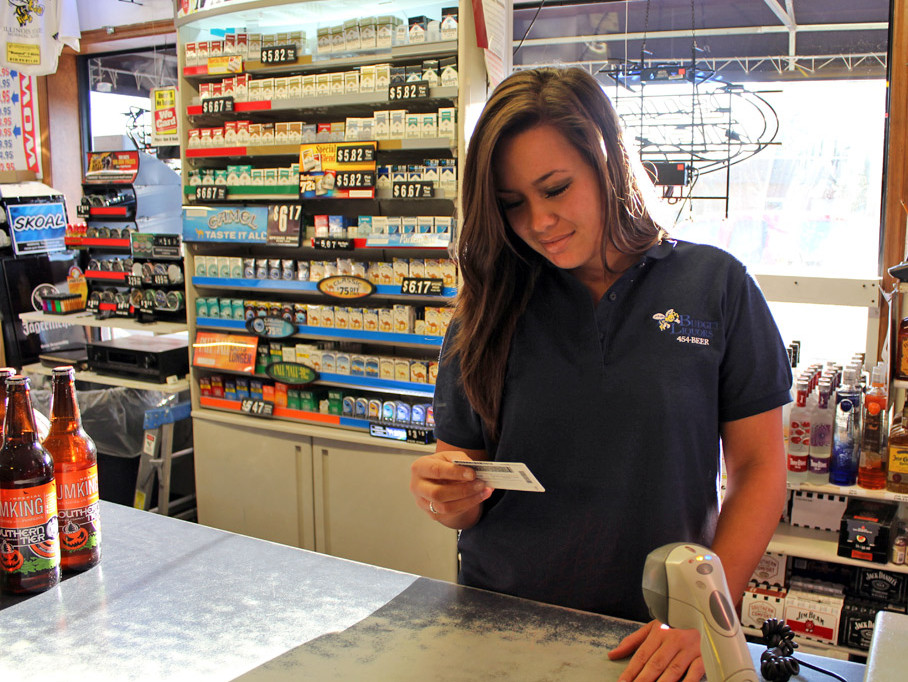
\includegraphics[height=\paperheight,width=\paperwidth]{images/UnderageAlcohol3.jpg}};
  \end{columns}
\end{frame}

\section{Theory}
\begin{frame}
  \frametitle{IRMA}
  \framesubtitle{Card}  
  \begin{itemize}
    \item Contactless smart card
    \item Outside only shows picture of card holder
  \end{itemize}
  
  \begin{figure}[tb]
    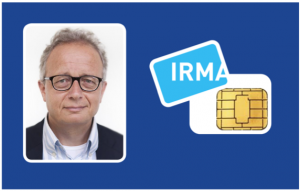
\includegraphics[width=0.35\textwidth]{images/IRMA_card_front.png}
    \hspace*{1mm}
    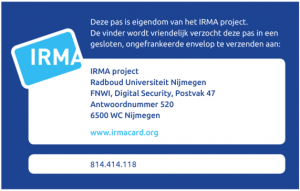
\includegraphics[width=0.35\textwidth]{images/IRMA_card_back.png}    
  \end{figure}
\end{frame}

\begin{frame}
  \frametitle{IRMA}
  \framesubtitle{Details}
  \begin{itemize}
    \item ``I Reveal My Attributes''
    \item Attribute-based credentials
    \item Authentication by verification of issuer signature
  \end{itemize}
  \begin{figure}[tb]
      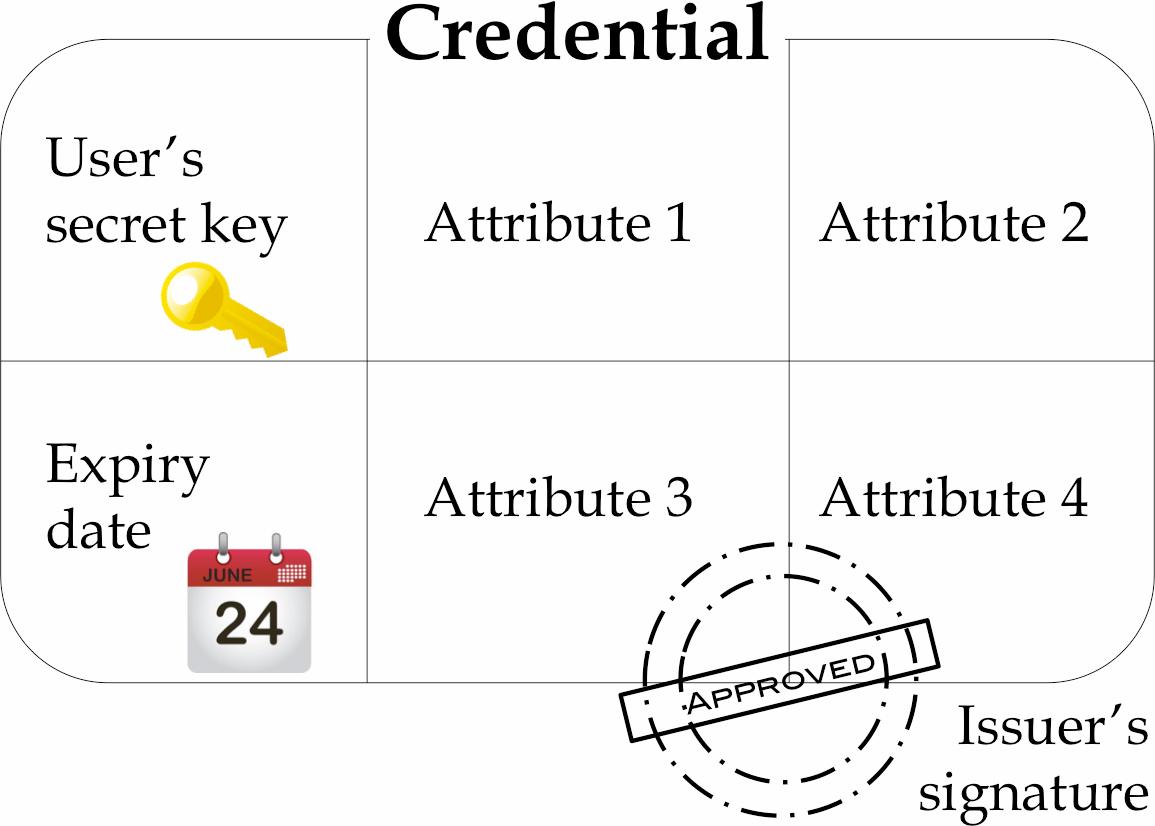
\includegraphics[width=0.3\textwidth]{images/ABC.png}
    \end{figure}
\end{frame}

\begin{frame}
  \frametitle{IRMA}
  \framesubtitle{Actors}
  \begin{itemize}
    \item Users
    \item Issuers
    \item Verifiers / relying parties
    \item Scheme manager
  \end{itemize}
\end{frame}

\begin{frame}
  \frametitle{Passport}
  \framesubtitle{Basic elements}
  \vspace*{-0.8cm}
  \begin{figure}[tb]
    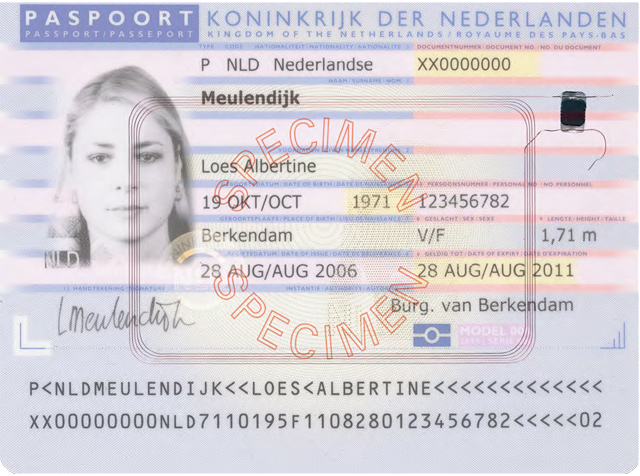
\includegraphics[width=0.35\textwidth]{images/dutchpassport.png}
  \end{figure}
  \begin{itemize}
    \item<1-> Name, date of birth, place of birth, height
    \item<2-> Biometrics (finger prints, iris scans)
  \end{itemize}
\end{frame}

\begin{frame}
  \frametitle{Passport}  
  \framesubtitle{Cryptography}
  \begin{itemize}
    \item Passive Authentication (PA)
    \item Basic Access Control (BAC)
    \item Secure Messaging (SM)
    \item Supplemental Access Control (SAC)
    \begin{itemize}
      \item Password Authenticated Connection Establishment (PACE)
    \end{itemize}
    \item Active Authentication (AA)
    \item Extended Access Control (EAC)
    \begin{itemize}
      \item Chip Authentication (CA)
      \item Terminal Authentication (TA)
    \end{itemize}
    \vspace*{0.6cm}
    \tikz[overlay,remember picture] 
    \node[opacity=0.3, at=(current page.south east),anchor=south east,inner sep=70pt]{
\includegraphics[width=0.1\textwidth]{images/biometrics_logo}};
  \end{itemize}  
\end{frame}

\section{Goals}
\begin{frame}
  \frametitle{Designing the protocol}
  \framesubtitle{Requirements}
  \begin{itemize}
    \item Mutual authentication between client and server
    \item Integrity of passport data
    \item Confidentiality of passport data
    \item Integrity of ABCs
    \item Confidentiality of ABCs
    \item Resistance against replay attacks
  \end{itemize}
\end{frame}

\begin{frame}
  \frametitle{Designing the protocol}
  \framesubtitle{Goals}
  \begin{block}{Goals}
    \begin{itemize}
      \item Authenticity
      \item Accountability
      \item Confidentiality
      \item Integrity
      \item \scriptsize Availability
    \end{itemize}
  \end{block}
\end{frame}

\section{Protocols}
\begin{frame}
  \frametitle{TLS}
  \framesubtitle{Basics}
  \begin{itemize}
    \item Transport Layer Security
    \item Two parts
    \begin{itemize}
      \item Handshake
      \item Record
    \end{itemize}
    \item Makes use of TCP
    \item Provides encryption and authentication
    \item At least version 1.2
    \begin{itemize}
      \item Perfect forward secrecy
    \end{itemize}
  \end{itemize}  
\end{frame}

\begin{frame}[fragile]
  \frametitle{TLS}
  \framesubtitle{Handshake}
\scriptsize
  \begin{semiverbatim}
{\large Client}                                     {\large Server}
------------                                   ------------
ClientHello              -------->
                                                ServerHello
                                               Certificate*
                                         ServerKeyExchange*                
                                        CertificateRequest*
                         <--------          ServerHelloDone
Certificate*
ClientKeyExchange
CertificateVerify*
[ChangeCipherSpec]
Finished                 -------->
                                         [ChangeCipherSpec]
                         <--------                 Finished
Application Data         <------->         Application Data
\end{semiverbatim}
\end{frame}

\begin{frame}
  \frametitle{IRMA Assurer (todo: wisselen met TLS?)}
  \framesubtitle{Basic course of events}
  
  \begin{enumerate}
    \item<1-> Fill out application for IRMA card and enclose a photo
    \item<2-> New IRMA card is created and sent to an assurer
    \item<3-> Go to assurer's office and bring your passport
    \item<4-> The assurer verifies the photos and reads the data on the passport chip
    \item<5-> This data is sent to a remote server for verification
    \item<6-> The server creates ABCs corresponding to the passport contents
    \item<7-> The assurer receives the ABCs and stores them onto the IRMA card
  \end{enumerate}
\end{frame}

\begin{frame}
  \frametitle{IRMA Assurer}
  \framesubtitle{Assumptions -- Operational}
  \begin{itemize}
    \item Clients only communicate with the (only) server
    \item Client has a tablet which is PIN protected and locked in a safe when not in use
    \item Client performs PA
    \item Server also performs PA, plus AA
    \item Server checks for invalid or revoked client certificates    
  \end{itemize}
\end{frame}

\begin{frame}
  \frametitle{IRMA Assurer}
  \framesubtitle{Assumptions -- Cryptographic}
  \begin{itemize}
    \item Communication between client and IRMA card not secured
    \item Clients are initialized with a keypair, a certificate and the server's FQDN
    \item Clients also are initialized with the server's public key for easy access
    \item ABCs are deleted immediately after a successful protocol run
    \item Ephemeral keys, preferably Elliptic Curve Cryptography
    \item No session resuming
  \end{itemize}
\end{frame}

\begin{frame}[fragile]
  \frametitle{IRMA Assurer}
  \framesubtitle{Assumptions}
  \begin{block}{Supported ciphers}
  \begin{verbatim}
TLS_ECDHE_RSA_WITH_AES_128_GCM_SHA256
TLS_ECDHE_ECDSA_WITH_AES_128_GCM_SHA256
TLS_ECDHE_RSA_WITH_AES_256_GCM_SHA384
TLS_ECDHE_ECDSA_WITH_AES_256_GCM_SHA384

TLS_ECDHE_RSA_WITH_AES_128_CBC_SHA256
TLS_ECDHE_ECDSA_WITH_AES_128_CBC_SHA256

TLS_ECDHE_RSA_WITH_AES_256_CBC_SHA384
TLS_ECDHE_ECDSA_WITH_AES_256_CBC_SHA384
  \end{verbatim}
  \end{block}
\end{frame}

\section{Formalisation}
\begin{frame}
\scriptsize
  \frametitle{Protocol}
  \framesubtitle{TLS and Assurer combined}
    \begin{enumerate}
      \listpart{\color{gray} Citizen presents passport \\ Client performs PA}
      \item A $\rightarrow$ B: ClientHello
      \item B $\rightarrow$ A: ServerHello, Certificate, ServerKeyExchange, CertificateRequest, ServerHelloDone
      \item A $\rightarrow$ B: Certificate, ClientKeyExchange, CertificateVerify, ChangeCipherSpec, \{Finished\}$_\text{kAB}$
      \item B $\rightarrow$ A: ChangeCipherSpec, \{Finished\}$_\text{kAB}$
      \item A $\rightarrow$ B: \{\{Passport, A, B, Na\}$_\text{kAB}$, \#\{Passport\}$_\text{kAB}$\}$_\text{kAB}$
      \listpart{\color{gray} Server performs PA}
      \item B $\rightarrow$ A $\rightarrow$ P: \{Nb\}$_\text{kAB}$
      \item P $\rightarrow$ A $\rightarrow$ B: \{\{Nb\}$_\text{skP}$\}$_\text{kAB}$
      \listpart{\color{gray} Server verifies response to AA challenge}
      \item B $\rightarrow$ A: \{\{ABCs, A, B, Na\}$_\text{kAB}$, \#\{ABCs\}$_\text{kAB}$\}$_\text{kAB}$
      \listpart{\color{gray} Client stores ABCs on IRMA card}
    \end{enumerate}
\end{frame}

\begin{frame}
  \frametitle{Model}
  \begin{block}{Model}
    \begin{itemize}
      \item 
    \end{itemize}
  \end{block}
\end{frame}

\section{Conclusion}
\begin{frame}
  \frametitle{Conclusion}
\end{frame}

\end{document}
